\newpage
\clearpage

\appendix



\begin{table*}[!t]
    % \aboverulesep = 0.48mm
    % \belowrulesep = 0.48mm
    \small
	\centering	
 \begin{tabular}	{l  |  c  c  c  }
        \toprule
        LLM & FlanT5$_\text{XL}$ & OPT$_\text{2.7B}$ & OPT$_\text{6.7B}$\\
        \midrule
        Fine-tuning epochs & \multicolumn{3}{c}{5}\\
        Warmup steps & \multicolumn{3}{c}{1000}\\
        Learning rate & \multicolumn{3}{c}{1e-5} \\
        Batch size & \multicolumn{3}{c}{256} \\
        AdamW $\beta$ & \multicolumn{3}{c}{(0.9,0.999)} \\
        Weight decay & \multicolumn{3}{c}{0.05}\\
        Drop path & \multicolumn{3}{c}{0}\\
        Image resolution & \multicolumn{3}{c}{364}\\
        Prompt & \multicolumn{3}{c}{``a photo of''}\\
        Inference beam size & \multicolumn{3}{c}{5}\\   
        Layer-wise learning rate decay for ViT & 1 & 1 & 0.95\\
 	\bottomrule	
	\end{tabular}

 \vspace{-1ex}
	\caption
	{
	\small	
        Hyperparameters for fine-tuning BLIP-2 with ViT-g on COCO captioning.
	}
	\vspace{-1ex}
\end{table*}	


\begin{table*}[!t]
    % \aboverulesep = 0.48mm
    % \belowrulesep = 0.48mm
    \small
	\centering	
 \begin{tabular}	{l  |  c  c  c  }
        \toprule
        LLM & FlanT5$_\text{XL}$ & OPT$_\text{2.7B}$ & OPT$_\text{6.7B}$\\
        \midrule
        Fine-tuning epochs & \multicolumn{3}{c}{5}\\
        Warmup steps & \multicolumn{3}{c}{1000}\\
        Learning rate & \multicolumn{3}{c}{1e-5} \\
        Batch size & \multicolumn{3}{c}{128} \\
        AdamW $\beta$ & \multicolumn{3}{c}{(0.9,0.999)} \\
        Weight decay & \multicolumn{3}{c}{0.05}\\
        Drop path & \multicolumn{3}{c}{0}\\
        Image resolution & \multicolumn{3}{c}{490}\\
        Prompt & \multicolumn{3}{c}{``Question: \{\} Answer:''}\\
        Inference beam size & \multicolumn{3}{c}{5}\\   
        Layer-wise learning rate decay for ViT & 0.95 & 0.95 & 0.9\\
 	\bottomrule	
	\end{tabular}

 \vspace{-1ex}
	\caption
	{
	\small	
        Hyperparameters for fine-tuning BLIP-2 with ViT-g on VQA.
	}
	\vspace{-1ex}
\end{table*}		 


\begin{table*}[!t]
    % \aboverulesep = 0.48mm
    % \belowrulesep = 0.48mm
    \small
	\centering	
 \begin{tabular}	{l  |  c  c  }
        \toprule
        Image Encoder & ViT-L/14 & ViT-g/14\\
        \midrule
        Fine-tuning epochs & \multicolumn{2}{c}{5}\\
        Warmup steps & \multicolumn{2}{c}{1000}\\
        Learning rate& 5e-6 & 1e-5  \\
        Batch size & \multicolumn{2}{c}{224} \\
        AdamW $\beta$ & (0.9,0.98) & (0.9,0.999) \\
        Weight decay & \multicolumn{2}{c}{0.05}\\
        Drop path & \multicolumn{2}{c}{0}\\
        Image resolution & \multicolumn{2}{c}{364}\\
        Layer-wise learning rate decay for ViT & 1 & 0.95\\
 	\bottomrule	
	\end{tabular}

 \vspace{-1ex}
	\caption
	{
	\small	
        Hyperparameters for fine-tuning BLIP-2 on COCO image-text retrieval.
	}
	\vspace{-1ex}
\end{table*}	


\begin{figure*}[b]
\centering
  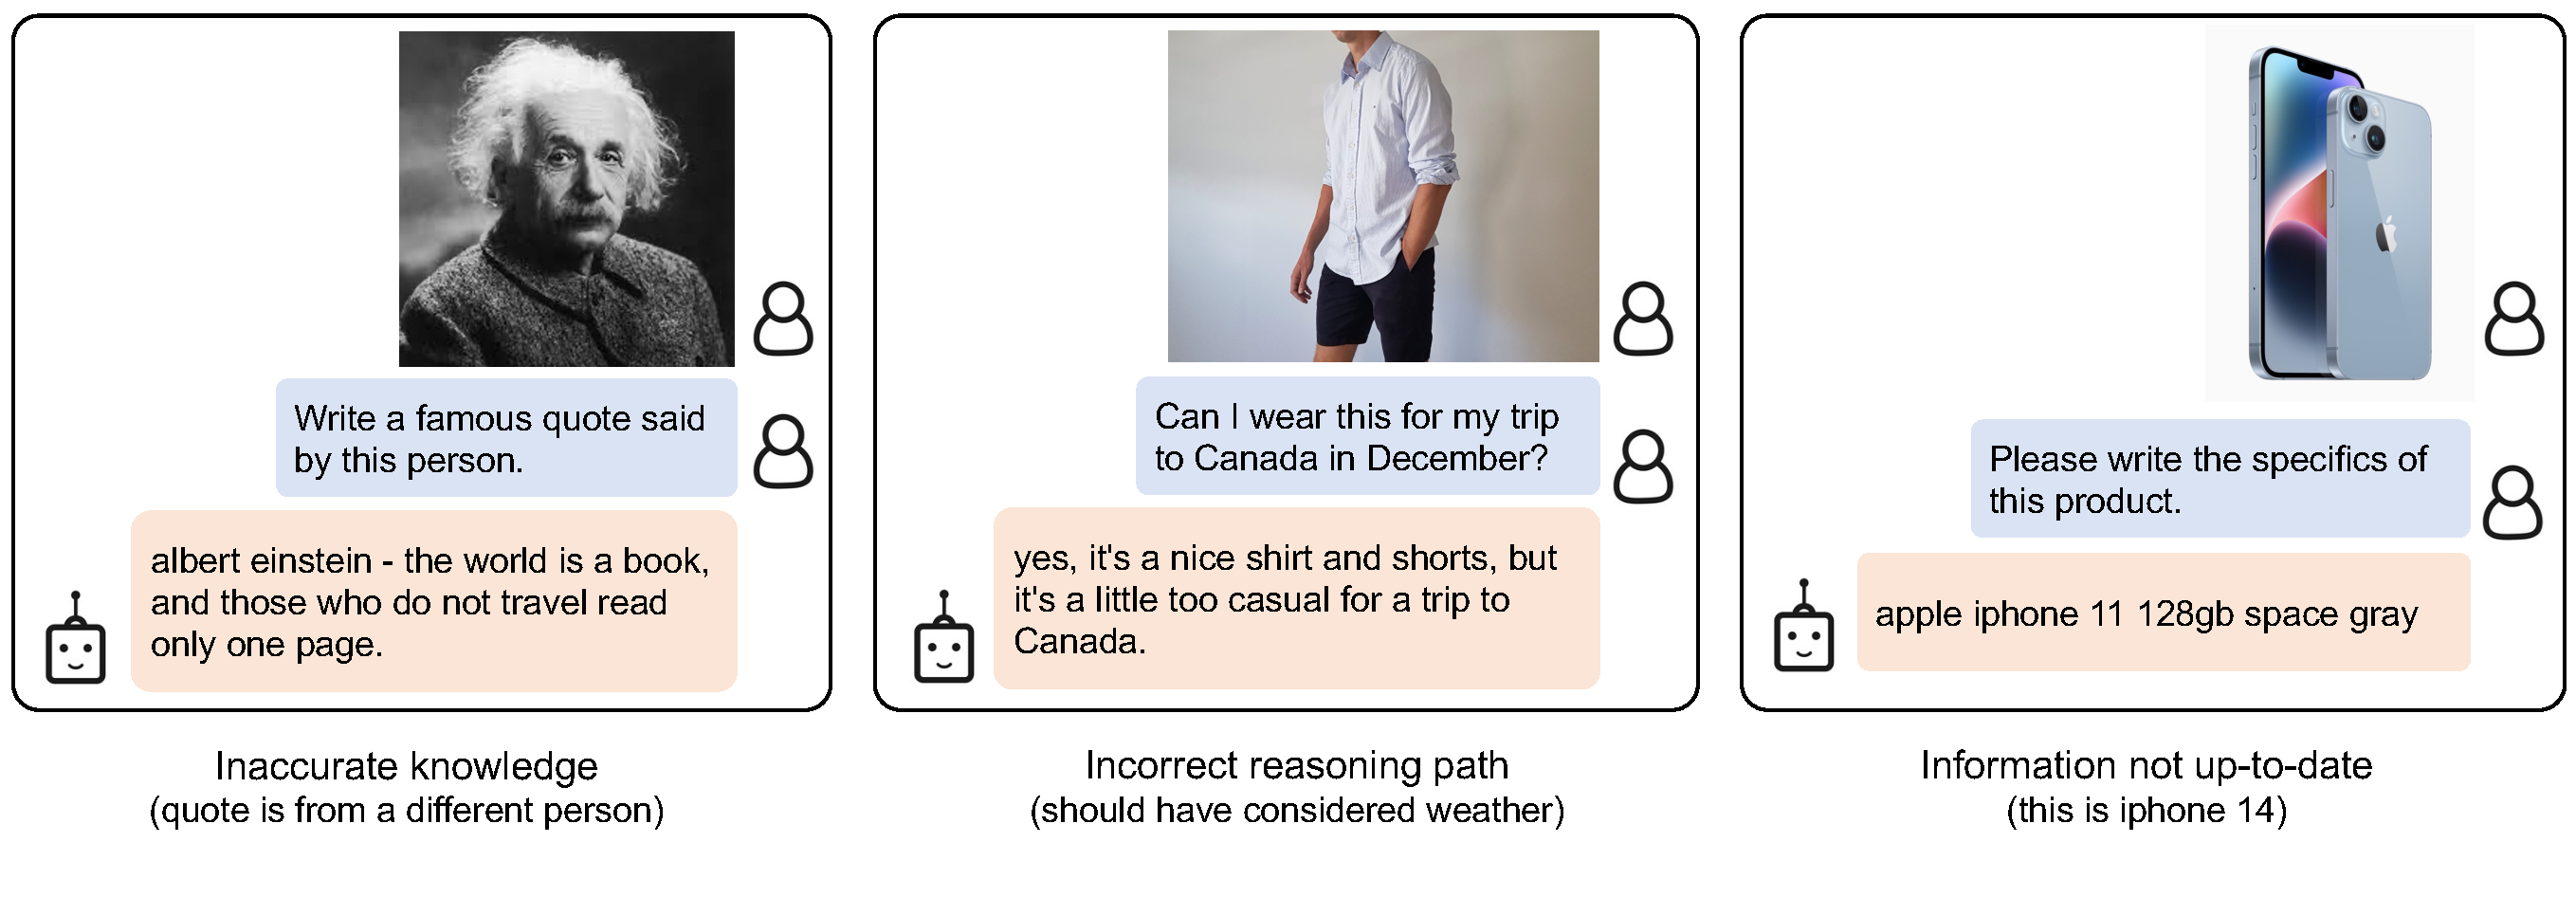
\includegraphics[width=\textwidth]{image/examples_limitation}
\vspace{-6ex}
\caption{Incorrect output examples for instructed zero-shot image-to-text generation using a BLIP-2 model w/ ViT-g and FlanT5$_\text{XXL}$.
% \DX{If I were to be picky, I could say this is not necessarily an out-of-date issue. Maybe the visual feature of iphone 11 and 14 just too similar. Maybe we can put a football world cup trophy and ask who won the most recent champion?}
}
%\vspace{-1ex}
\clearpage
\label{fig:example_limitation}
\end{figure*}

\begin{figure}[t!]
\centering
  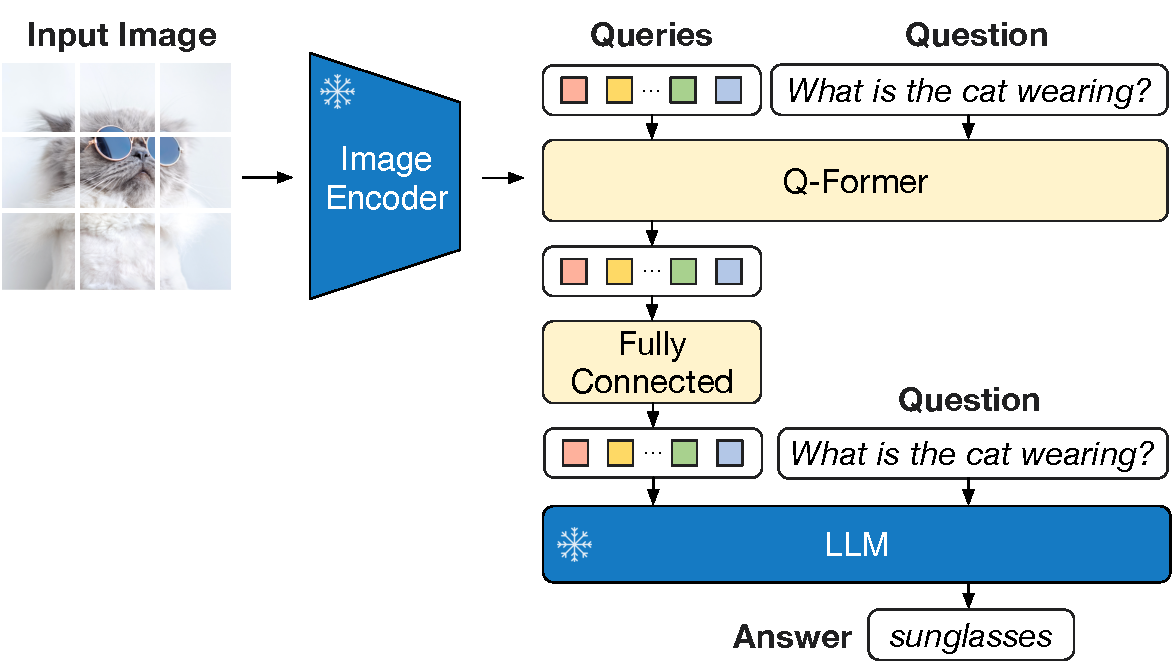
\includegraphics[width=0.48\textwidth]{image/fig-vqa.pdf}
% \vspace{-6ex}
\caption{Model architecture for VQA finetuning, where the LLM receives Q-Former's output and the question as input, then predicts answers. We also provide the question as a condition to Q-Former, such that the extracted image features are more relevant to the question.
}
%\vspace{-1ex}
\label{fig:example_limitation}
\end{figure}
